\chapter {سیستم گراف پویانمایی در موتور بازی‌سازی آنریل}

موتور آنریل مجموعه کاملی از ابزار‌های تولید محتوا برای توسعه‌ی بازی، مصورسازی معماری و خودرو، 
ایجاد محتوا برای فیلم و تلوزیون،
پخش رویداد‌های زنده، آموزش، شبیه‌سازی 
و سایر برنامه‌های بلادرنگ است.

این موتور برای اولین بار برای توسعه‌ی بازی "غیرواقعی" در سال 1998 توسعه پیدا کرد.
پس از آن نسخه‌های متعددی از این موتور منتشر شده است.
\cite{UnrealEngineWikiPedia}

موتور آنریل مانند تمامی موتور‌های بازی‌سازی دارای مولفه‌های فراوانی است که برای 
تولید بازی به کار می‌رود.
مولفه‌های پویانمایی، هوش مصنوعی، رندر، رابط کاربری تنها تعداد اندکی از مولفه‌هایی است که ‌می‌توان در 
آنریل استفاده کرد.

آنریل طیف گسترده‌ای از ابزار‌های قدرتمند را برای مدیریت شخصیت‌ها، ایجاد محتوای سینمایی 
و پویانمایی را ارائه می‌دهد.
با استفاده از سیستم پویانمایی مش اسکلتی، 
کاربران می‌توانند شخصیت‌ها، اسکلت‌ها و کلیپ‌های پویانمایی 
وارد شده خود را مدیریت کنند.
سپس این محتوا می‌تواند برای ایجاد گیم‌پلی تعاملی پویا شده با استفاده از 
ویژگی‌های مختلف مانند 
فضا‌های ترکیبی 
\LTRfootnote{Blend Spaces}
، طرح‌های پویانمایی 
\LTRfootnote{Animation Blueprint}
و ماشین‌های حالت 
\LTRfootnote{State Machines}
استفاده شود.
سکانس‌های سینمایی را می‌توان با استفاده از ابزار 
\lr{Sequencer}
ایجاد کرد. با استفاده از این ابزار می‌توان 
دوربین‌ها و شخصیت‌ها را متحرک ساخت.
پویانمایی شخصیت‌ها را می‌توان با استفاده از 
\lr{Control Rig}
که ابزار داخلی 
موتور آنریل است، انجام داد.
با استفاده از این ابزار می‌توان ریگ‌های مناسبی ساخت تا 
درون 
\lr{Sequencer}
شخصیت را متحرک ساخت.
\cite{UnrealEngineAnimation}

همانطور که مشخص است، سیستم پویانمایی موجود در موتور آنریل بسیار گسترده است. در این پروژه 
قسمت طرح پویانمایی آنریل که به گراف پویانمایی نیز شناخته می‌شود بررسی می‌شود.

برای اینکه بتوانیم در مورد سیسیتم گراف پویانمایی آنریل توضیح دهیم، ابتدا لازم است 
توضیحاتی را درباره‌ی نحوه‌ی معماری این انجین بیاوریم. بنابراین در این بخش ابتدا توضیح کوتاهی 
درباره‌ی معماری آنریل با محوریت نحوه‌ی رابطه‌‌ی اشیا با یکدیگر داده و 
پس از آن به بررسی ویژگی‌های سیستم گراف پویانمایی می‌پردازیم.

 
\section{بازیگران، پیاده‌ها و شخصیت‌‌ها}

اشیا در آنریل به سه کلاس کلی بازیگران
\LTRfootnote{Actors}
، پیاده‌ها 
\LTRfootnote{Pawns}
و شخصیت‌ها
\LTRfootnote{Characters}
دسته‌بندی می‌شوند.

بازیگران کلاس پایه‌ی تمامی اشیا ای هستند که به صورت فیزیکی می‌توانند در محیط سه‌بعدی قرار گیرند.
پیاده‌ها کلاسی مشتق شده از بازیگران هستند که بازیکنان می‌توانند کنترل آن‌ها را بدست گیرند و 
در محیط حرکت کنند.
 در نهایت شخصیت‌ها پیاده‌هایی هستند که دارای مش اسکلتونی، توانایی شناسایی برخورد و منطق حرکتی هستند.
 آنها مسئول تمام تعاملات فیزیکی بین بازیکن یا هوش مصنوعی، با جهان هستند و همچنین مدل های اولیه شبکه و دریافت ورودی را پیاده سازی می کنند. 
اگر بخواهیم شخصیت درون بازی از پویانمایی اسکلتونی استفاده کند، باید از این کلاس بهره ببریم.

\section{اجزاء}

اجزاء
\LTRfootnote{Components}
مجموعه‌ای از توابع و ویژگی‌ها است که می‌تواند به یک بازیگر اضافه شود.
بنابراین بازیگران می‌توانند حاوی مجموعه‌ای از
\lr{ActorComponents}
باشند که این اجزاء می‌توانند برای موارد مختلفی از جمله
کنترل نحوه‌ی حرکت بازیگران، 
نحوه‌ی رندر شدن و غیره استفاده شوند.

زمانی که یک مولفه به یک بازیگر اضافه می‌شود، آن بازیگر می‌تواند عملکرد‌های موجود در آن مولفه را استفاده کند.
به عنوان مثل یک مولفه نور نقطه‌ای باعث می‌شود که بازیگر مانند یک نور نقطه‌ای، نور ساطع کند.
یا یک مولفه صوتی به بازیگر این توانایی پخش صدا را می‌دهد.

مولفه‌ها حتما باید به یک بازیگر متصل شوند و به خودی خود نمی‌توانند وجود داشته باشند.
درواقع وقتی ما مولفه‌های مختلف را به بازیگر خود متصل می‌کنیم، در حال قرار دادن قطعه‌ها و تکه‌هایی هستیم
 که مجموع آن‌ها یک بازیگر را به عنوان یک موجودیت واحد که در محیط سه‌بعدی قرار می‌گیرد، تعریف می‌کنند.
 به عنوان مثال چرخ‌های یک ماشین، فرمان ماشین، چراغ‌ها و غیره همه به عنوان
 مولفه‌های ماشین درنظر گرفته می‌شوند در حالی که خود آن ماشین، بازیگر است.

\section{شخصیت‌ها}

هر شخصیت در آنریل از سه مولفه‌ی اصلی تشکیل شده است.


\begin{itemize}
	\item[-] \lr{Skeletal Mesh Component}
	\item[-] \lr{Character Movement Component}
	\item[-] \lr{Capsule Component}
\end{itemize}


مولفه‌ی 
\lr{Skeletal mesh Component }
شامل طرح پویانمایی شخصیت است. طرح پویانمایی، سیستم پویانمایی شخصیت است که جلوتر آن را توضیح می‌دهیم.


مولفه‌ی 
\lr{ Character Movement Component}
همانطور که از اسمش مشخص است برای منطق حرکت در حالت‌های مختلف از جمله راه‌رفتن، افتادن و غیره استفاده می‌شود.
این مولفه شامل تنظیمات و عملکرد‌های مربوطه برای کنترل حرکت است.

و در نهایت مولفه‌‌ی
\lr{Capsule Component}
وظیفه‌ی تشخیص برخورد در هنگام حرکت را دارد.


\section{مولفه‌ی مش اسکلتی}

این مولفه‌، مولفه‌ای است که به شخصیت امکان پویا شدن را می‌دهد.
این کلاس برای ساختن یک نمونه از کلاس 
\lr{SkeletalMesh}
است که بر روی آن کلیپ‌های پویانمایی اجرا می‌شوند.
اینکه چه کلیپ پویانمایی بر روی آن اجرا شود از طریق کلاس 
\lr{AnimInstance}
که همان طرح پویانمایی
\LTRfootnote{Animation Blueprint}
 است، انتخاب می‌شود.

همانطور که در فصل گذشته اشاره شد، مش اسکلتی 
شامل یک هندسه‌ی چندضلعی است که به یک اسکلت که در واقع 
سلسله مراتبی از مفاصل است، متصل است و این اسکلت می‌تواند به 
منظور تغییر شکل آن هندسه‌ی چندضلعی یا مش، متحرک شود.

مش‌های اسکلتی از دو قسمت ساخته‌شده‌اند. مجموعه‌ای از چندضلعی‌ها
که به منظور تشکیل سطح مش با یکدیگر ترکیب می‌شوند و 
یک اسکلت سلسله‌مراتبی که می‌تواند برای متحرک‌سازی چند‌ضلعی‌ها استفاده شود.
مدل‌های سه‌بعدی، 
اسکلت
و کلیپ‌های پویانمایی 
در یک برنامه مدل‌سازی و ایجاد پویانمایی
مانند 
\lr{Maya}،
\lr{3DSMax}
و ابزار‌های مدل‌سازی دیگر ایجاد می‌شوند.

در آنریل کلاس 
\lr{SkeletalMesh}
وظیفه‌ی نگهداری این مش اسکلتی را دارد.

همانگونه که گفتیم، نیاز داریم تا یک سیستمی داشته باشیم 
که بتواند کلیپ‌های پویانمایی را بر روی 
این مش اسکلتی اجرا کند. به زبانی دیگر، این 
مش اسکلی را پویا و متحرک سازد.
در آنریل کلاس 
\lr{AnimInstance}
وظیفه‌ی این عمل را دارد.

\section{طرح پویانمایی}

طرح پویانمایی یک طرح تخصصی است که پویانمایی 
یک مش اسکلتی را کنترل می‌کند.
با ویرایش گراف‌های موجود در این طرح، 
میتوان کار‌های مختلفی را روی پویانمایی شخصیت انجام داد.
به عنوان مثال می‌توان کلیپ‌های مختلف را با یکدیگر ترکیب کرد،
مستقیما مفاصل درون اسکلت را کنترل کرد و
یا هر تنظیمات منطقی‌ای که باعث تعریف 
ژست نهایی شخصیت در فریم فعلی می‌شود را انجام داد.

دو جزء اصلی در طرح پویانمایی وجود دارد که با هم کار می‌کنند تا ژست نهایی شخصیت را برای هر 
فریم ایجاد کنند.
این دو مولفه، گراف رویداد و گراف پویانمایی نام دارند.

به صورت کلی گراف رویداد مقادیری را که در گراف پویانمایی استفاده می‌شوند را به‌روز‌رسانی می‌‌کند تا 
در ماشین‌های حالت، فضاهای ترکیب و بقیه‌ی گره‌هایی که در گراف پویانمایی
 استفاده می‌شوند، به کار روند.

\section{گراف رویداد}

درون هر طرح پویانمایی، یک گراف رویداد وجود دارد. 
این گراف برای دریافت مقادیر منطقی از بخش گیمپلی و منطق بازی به‌کار می‌رود.
به عنوان مثال اینکه شخصیت می‌خواهد به چه سمتی حرکت کند، یا اینکه چه سرعتی دارد را 
از طریق این گراف در متغیرهایی که تعریف می‌کنیم، ذخیره می‌کنیم.
\cite{EventGraphUnrealEngine}

\begin{figure}[ht]
	\centerline{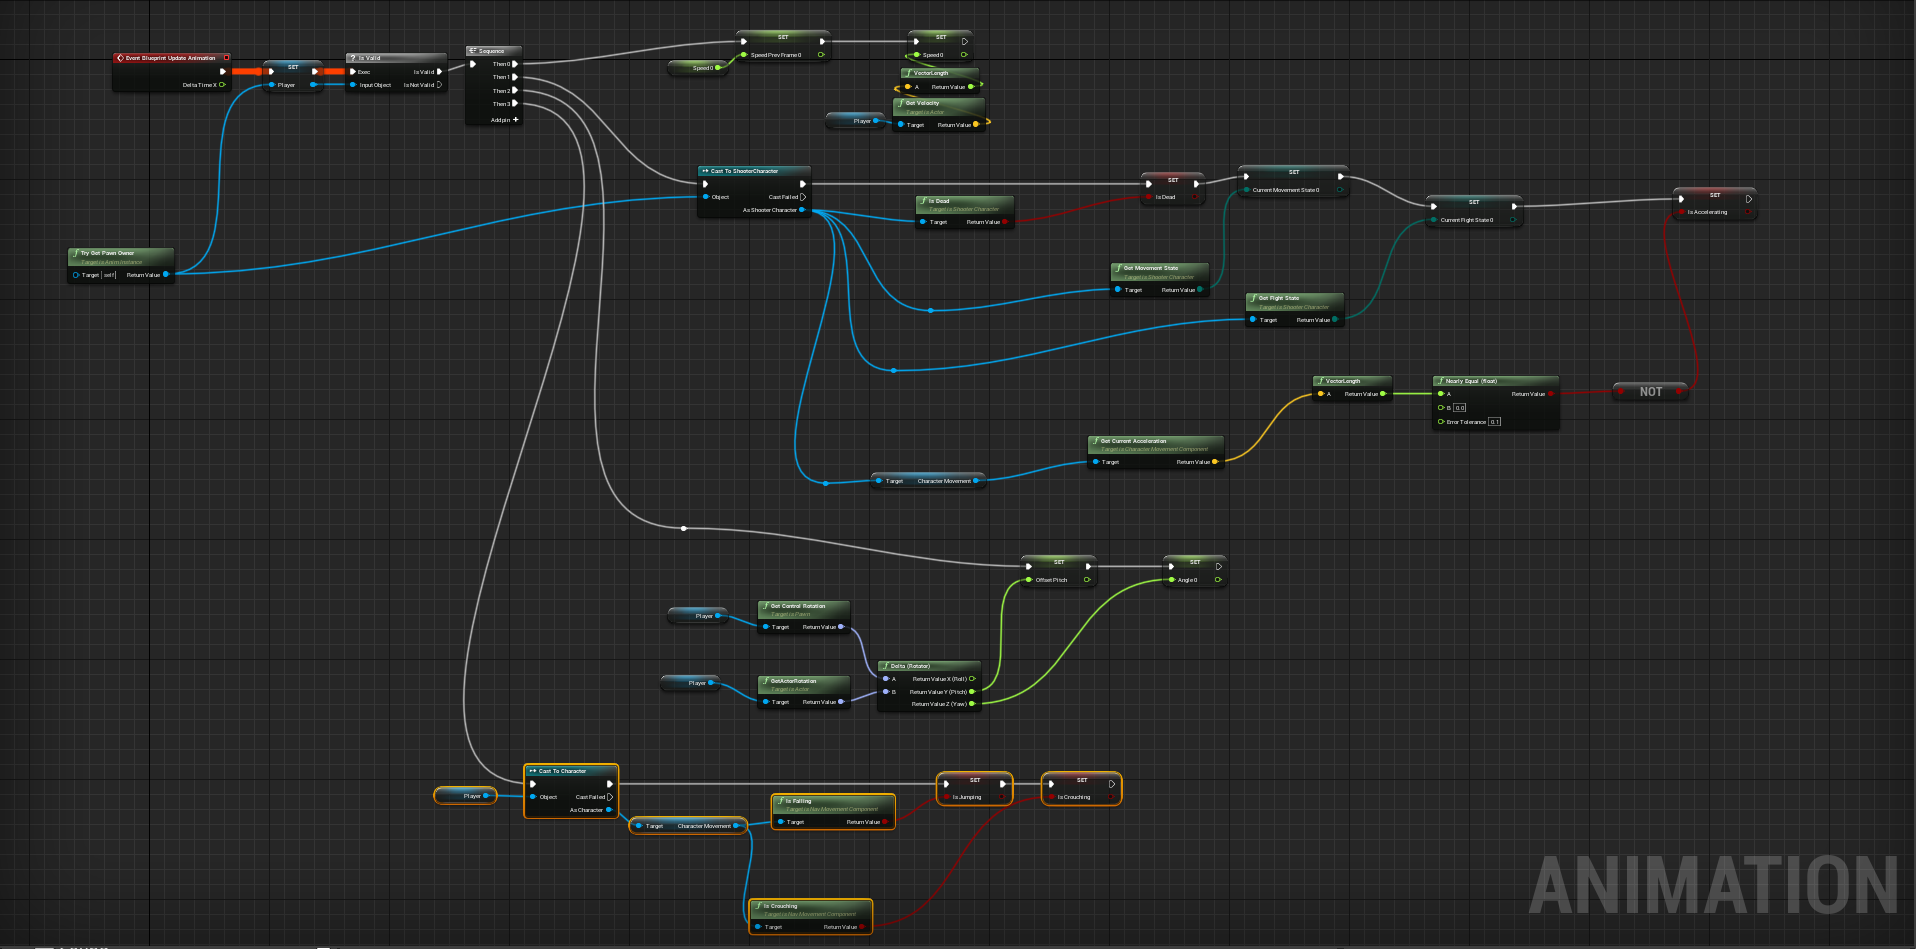
\includegraphics[width=\textwidth,height=8cm,keepaspectratio]{Figures/Ch3/EventGraph.png}}

	\caption{نمونه‌ای از یک گراف رویداد}
	\label{fig:EventGraph}
\end{figure}


\section{گراف پویا‌نمایی}

گراف پویانمایی برای ارزیابی ژست نهایی مش اسکلتی در فریم فعلی استفاده می‌شود.
به صورت کلی هر طرح پویانمایی دارای یک گراف پویانمایی است که 
این گراف شامل گره‌های مختلفی است که هر کدام از این گره‌ها استفاده‌های متفاوتی دارند.
به عنوان مثال می‌توان از این گره‌ها برای نمونه‌برداری


\begin{figure}[ht]
	\centerline{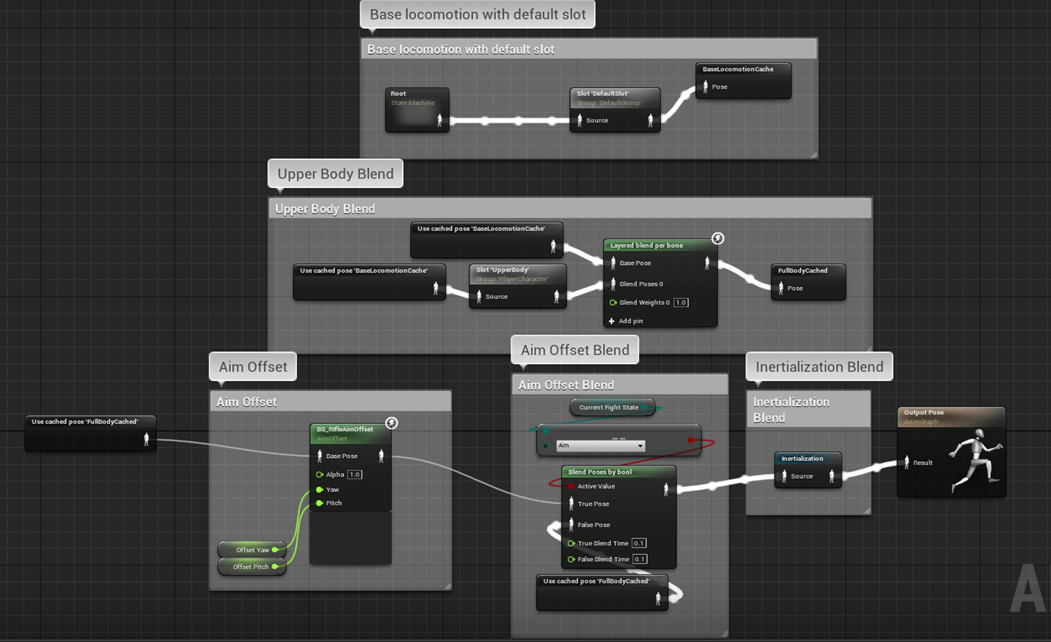
\includegraphics[width=\textwidth,height=8cm,keepaspectratio]{Figures/Ch3/AnimationGraph.png}}

	\caption{نمونه‌ای از یک گراف پویانمایی}
	\label{fig:AnimationGraph}
\end{figure}





\LTRfootnote{Sampling}
از دنباله‌های کلیپ‌های پویانمایی،
انجام ترکیب‌های بین کلیپ‌ها 
یا کنترل تبدیل‌های مربوط به مفاصل استفاده کرد.
سرانجام ژست نهایی بدست آمده روی 
مش اسکلتی در پایان هر فریم اعمال می‌شود.

\section{گره‌های گراف پویانمایی }

گراف پویا‌نمایی با ارزیابی گره‌های موجود در گراف، عمل می‌کند.
بعضی از گره‌های موجود در گراف، عملیات‌های خاصی را بر روی یک یا چند
ژست ورودی انجام می‌دهند، در حالی که برخی دیگر 
برای دسترسی یا نمونه‌برداری از انوع دیگری از دارایی‌ها مانند
فضاهای ترکیب
\LTRfootnote{Blend Spaces}
، مونتاژهای پویانمایی
\LTRfootnote{Animation Montages}
و دنباله‌های پویا‌نمایی
\LTRfootnote{Animation Sequence}
استفاده می‌شوند.
ماشین‌های حالت نیز که حاوی شبکه‌ی نموداری خودشان هستند، می‌توانند 
به صورت تنهایی یا با ترکیب با یکدیگر در 
گراف پویانمایی استفاده شوند.

در این بخش ابتدا با نحوه‌‌ی جریان اجرا در گراف پویانمایی 
آشنا می‌شویم، سپس ساختار کلی گره‌های موجود را بررسی کرده و در نهایت 
به بررسی انواع گره‌‌های موجود در گراف پویانمایی می‌پردازیم.



\section{ساختار گره‌های گراف پویانمایی}

گره‌‌ها می‌توانند شامل چند پین ورودی که درواقع ژست‌های ورود هستند، باشند.
به صورت کلی پین‌ها شامل یک خروجی هستند که این خروجی نشان‌دهنده‌ی 
ژست شخصیت پس از انجام عملیات‌های مربوط به آن پین است.
همچنین می‌توانند شامل پین‌های ویژگی باشند. مقادیر این پین‌های ویژگی از 
متغیر‌هایی که در گراف رویداد تعریف و مقداردهی شده‌اند، می‌توانند بدست آیند.

\begin{figure}[ht]
	\centerline{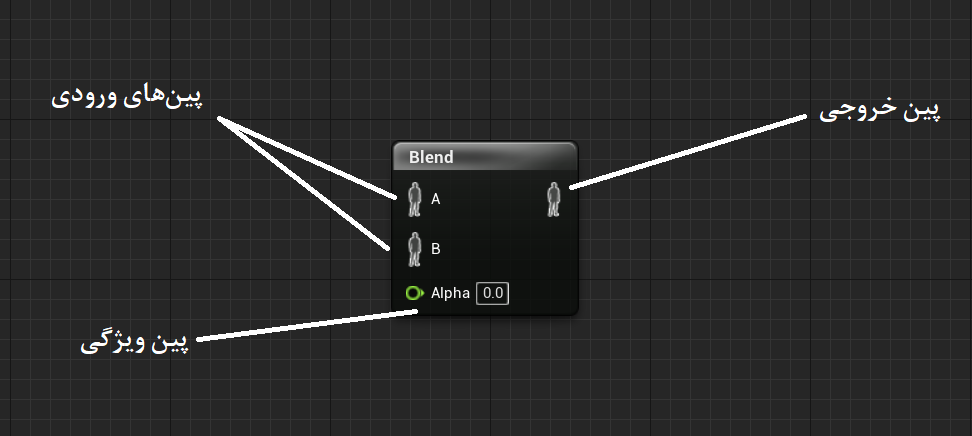
\includegraphics[width=\textwidth,height=8cm,keepaspectratio]{Figures/Ch3/AnimNodeStructure.png}}

	\caption{ساختار کلی گره‌های موجود در گراف پویانمایی}
	\label{fig:AnimNodeStructure}
\end{figure}

قابل ذکر است با انتخاب هر گره می‌توان به پنل جزئیات آن هم دسترسی پیدا کرد 
که به وسیله‌ی‌ آن می‌توان تنظیمات لازم را بر روی آن گره انجام داد.

\begin{figure}[ht]
	\centerline{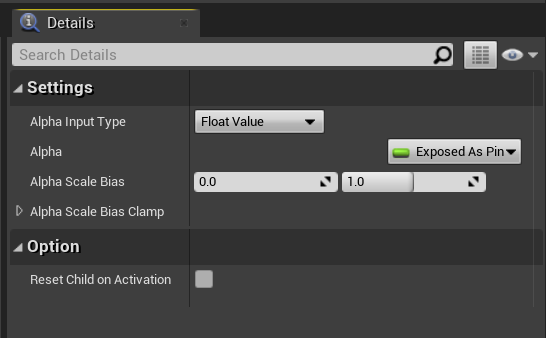
\includegraphics[width=\textwidth,height=8cm,keepaspectratio]{Figures/Ch3/DetailsPanel.png}}

	\caption{پنل تنظیمات گره‌ی ترکیب}
	\label{fig:AnimNodeDetailPanel}
\end{figure}

\section{جریان اجرا در گراف پویانمایی}

تمامی گراف‌ها دارای یک جریان اجرا هستند که به صورت پیوند‌های ضربانی 
میان ورودی و خروجی پین‌ها قابل مشاهده هستند. این جریان‌ها درواقع نحوه‌ی حرکت داده
را در گراف ترسیم می‌کنند.
در گراف پویانمایی، این جریان نشان‌دهنده‌ی ‌ژست‌هایی است که از 
یک گره به گره‌ی دیگر منتقل می‌شود.
در برخی از گره‌‌ها مانند گره‌ی ترکیب، ورودی‌های متعددی وجود دارند و به صورت 
درونی با مقادیری که در متغیر‌ها داریم تصمیم می‌گیرند که کدام یک از ورودی‌‌ها 
در حال حاضر بخشی از جریان اجرا است.


\begin{figure}[ht]
	\centerline{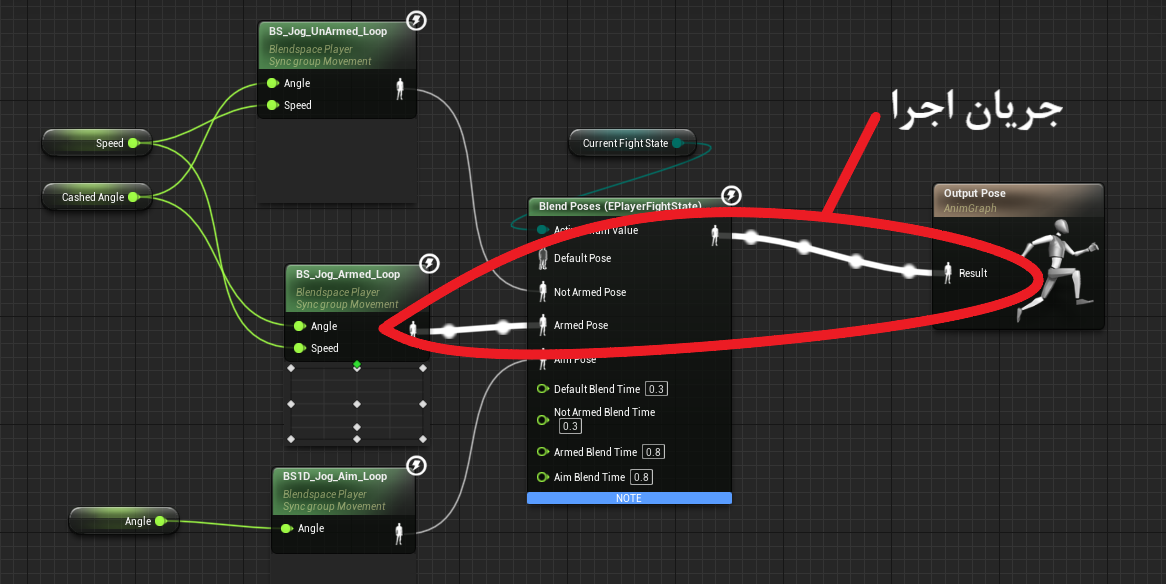
\includegraphics[width=\textwidth,height=8cm,keepaspectratio]{Figures/Ch3/ExecFlow.png}}

	\caption{نمونه‌ای از جریان اجرا}
	\label{fig:ExecFlow}
\end{figure}



\cite{AnimationGraphUnrealEngine}

\section {دنباله‌ی پویانمایی}

کلیپ‌های پویانمایی در آنریل به اسم دنباله‌ی پویانمایی شناخته می‌شوند.
دنباله‌ی پویانمایی یک دارایی پویانمایی است که 
حاوی داده‌‌های پویانمایی است که می‌تواند روی 
یک مش اسکلتی پخش شود تا شخصیت مربوط 
به آن اسکلت را متحرک سازد.
یک دنباله‌ی پویانمایی شامل فریم‌های کلیدی هستند که 
این فریم‌های کلیدی بیانگر موقعیت
\LTRfootnote{Position}
، دوران 
\LTRfootnote{Rotation}
، مقیاس
\LTRfootnote{Scale}
اسکلت مش در نقطه‌‌ی خاصی از زمان است.
بنابراین کلیپ‌های پویانمایی یکی از گره‌های مهم در 
گراف انیمشن حساب می‌آیند.

قابل ذکر است این گره‌ مانند بقیه‌ی گره‌ها دارای تنظیماتی است که در پنل تنظیمات قابل مشاهده‌ هستند. به عنوان مثال 
می‌توان سرعت حرکت کلیپ را در این تنظیمات مشخص کرد یا اینکه کلیپ به صورت حلقه‌وار تکرار شود یا خیر.

\begin{figure}[ht]
	\centerline{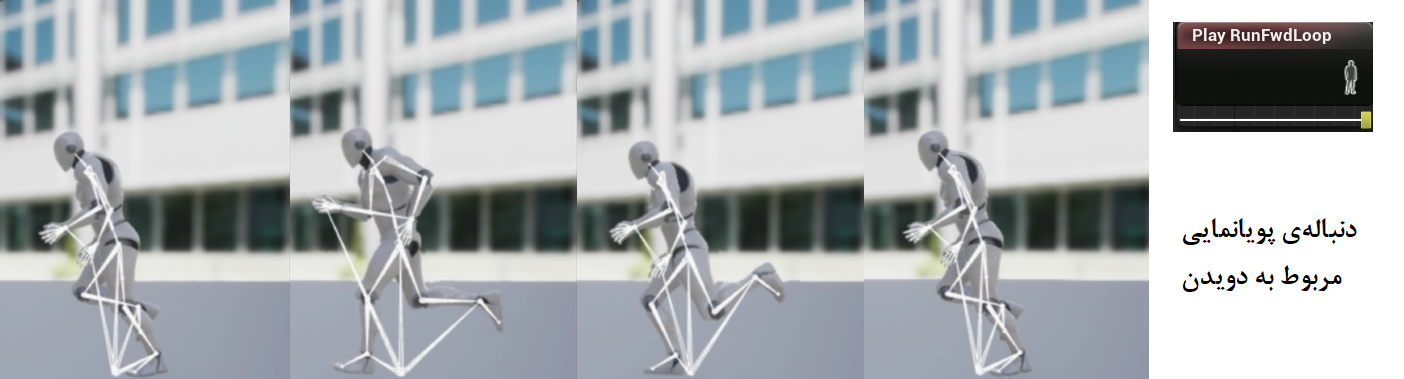
\includegraphics[width=\textwidth,height=8cm,keepaspectratio]{Figures/Ch3/AnimationSequence.png}}

	\caption{نمونه‌ای از گره‌ی دنباله‌ی پویانمایی}
	\label{fig:AnimationSequence}
\end{figure}



\section {فضای ترکیب}

فضای ترکیب یک دارایی به خصوص است که 
امکان ترکیب کلیپ‌های پویانمایی بر اساس مقدار مختلف ورودی را دارد.

به عنوان مثال فرض کنیم که چند کلیپ داریم که 
وضعیت حرکت شخصیت را مشخص می‌کنند.
این کلیپ‌ها می‌توانند به 
حالت ایستاده، حرکت با سرعت کم، حرکت با سرعت متوسط 
و حرکت با سرعت سریع تقسیم شوند.
علاوه‌ بر این‌ها می‌توان این پویانمایی‌ها را برای جهت‌های مختلف داشت.
در این صورت می‌توان یک فضای ترکیب داشت که بر اساس 
دو ورودی، سرعت و جهت عمل می‌کند.
و می‌توان هرکدام از این کلیپ‌ها را در جای مشخص خودش 
(با توجه به سرعت و جهت)
قرار داد.

درجلوتر اشاره می‌شود که می‌توان کلیپ‌ها را با استفاده از 
گره‌ی ترکیب نیز، با یکدیگر ترکیب نمود. 
فضای ترکیب، ابزاری برای انجام ترکیب‌های پیچیده‌تر 
بین کلیپ‌های پویانمایی متعدد بر اساس 
مقادیر متفاوت است.
هدف این گره، کاهش نیاز به ایجاد گره‌های منفرد
در هنگامی که می‌خواهیم ترکیب بر اساس ویژگی‌ها یا شرایط خاصی 
صورت گیرد، است.


\begin{figure}[ht]
	\centerline{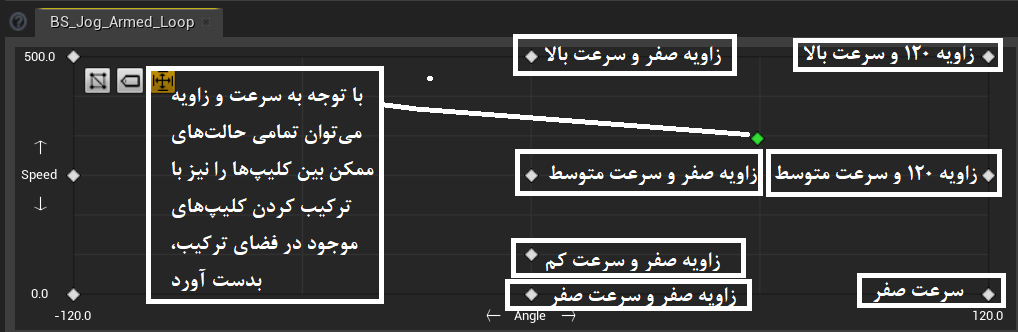
\includegraphics[width=\textwidth,height=8cm,keepaspectratio]{Figures/Ch3/BlendSpace.png}}

	\caption{در این فضای حالت، سرعت بین 0 تا 500 متغیر است و زاویه بین -120 تا 120 متغیر است.(در شکل به صورت کمی نوشته‌شده‌است)
	در کل از 10 کلیپ پویانمایی شده (نقاط سفیدرنگ در تصویر) ولی با استفاده از ترکیب بین این کلیپ‌ها می‌توان تمامی مقادیر بین کلیپ‌ها را نیز بدست آورد. }
	\label{fig:BlendSpace}
\end{figure}


\section {گره‌های ترکیب}

گره‌های ترکیب برای ترکیب چندین کلیپ پویانمایی با یکدیگر استفاده‌ می‌شوند.
این گره‌‌ها تنها مختص گراف پویانمایی هستند و در گراف‌های دیگر مانند گراف رویداد 
نمی‌توان از آن‌ها استفاده کرد.
به صورت کلی هر کدام از این نوع گره‌ها دارای چند پین ورودی و 
یک آلفا یا وزن است که برای محاسبه‌ی 
وزن هرکدام از ژست‌های ورودی در ژست خروجی به کار می‌رود.
بعضی از این گره‌‌ها می‌توانند 
پیچیده‌تر نیز باشند و نیاز به داده‌های بیشتری به عنوان ورودی باشند.

در ادامه به بررسی چند نمونه از گره‌‌های ترکیب می‌پردازیم.

\subsection{ گره‌ی ترکیب استاندارد}

این گره برای ترکیب‌کردن دو ژست ورودی با گرفتن یک آلفا عمل می‌کند.
اگر ژست‌های ورودی را
\lr{A}
و 
\lr{B}
 و
خروجی نهایی را 
\lr{Output}
در نظر بگیریم، 
خروجی به صورت زیر محاسبه می‌شود.

\begin{equation}\label{eq:BlendNode}
	Output= A * (1-alpha) + B * alpha
\end{equation}

\cite{BlendNodeUnrealEngine}

\begin{figure}[ht]
	\centerline{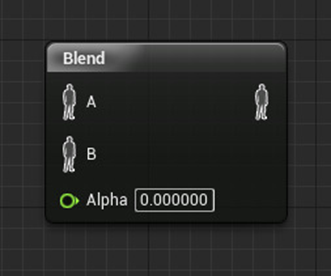
\includegraphics[width=\textwidth,height=8cm,keepaspectratio]{Figures/Ch3/BlendNode.png}}\hfill
	\caption{ گره‌ی ترکیب }
	\label{fig:BlendNode}
\end{figure}

\subsection{ گره‌ی ترکیب بر اساس یک مقدار}

این نوع از گره‌ها برای ترکیب کلیپ‌های پویانمایی بر اساس یک مقدار 
که این مقدار می‌تواند عدد صحیح، مقدار بولین و یا مقداری از 
نوع داده‌ی 
\lr{Enum}
باشد.

به عنوان مثال فرض کنیم شخصیت درون بازی می‌تواند در وضعیت‌های مختلفی از نظر
حالت مبارزه با اسلحه قرار گیرد. این حالت‌ها می‌توانند حالت بدون اسلحه، 
حالت با اسلحه و حالت گرفتن نشانه با اسلحه باشد.
می‌توان این حالت‌ها را با
\lr{enum}
نشان داد.
اگر برای هرکدام از این حالات یک کلیپ پویانمایی داشته باشیم و بخواهیم 
با توجه به حالت فعلی شخصیت یکی از این کلیپ‌ها را روی شخصیت پخش کنیم،
می‌توانیم از این گره استفاده کنیم.
\cite{BlendNodeUnrealEngine}

این مثال در شکل زیر آمده است.

\begin{figure}[ht]
	\centerline{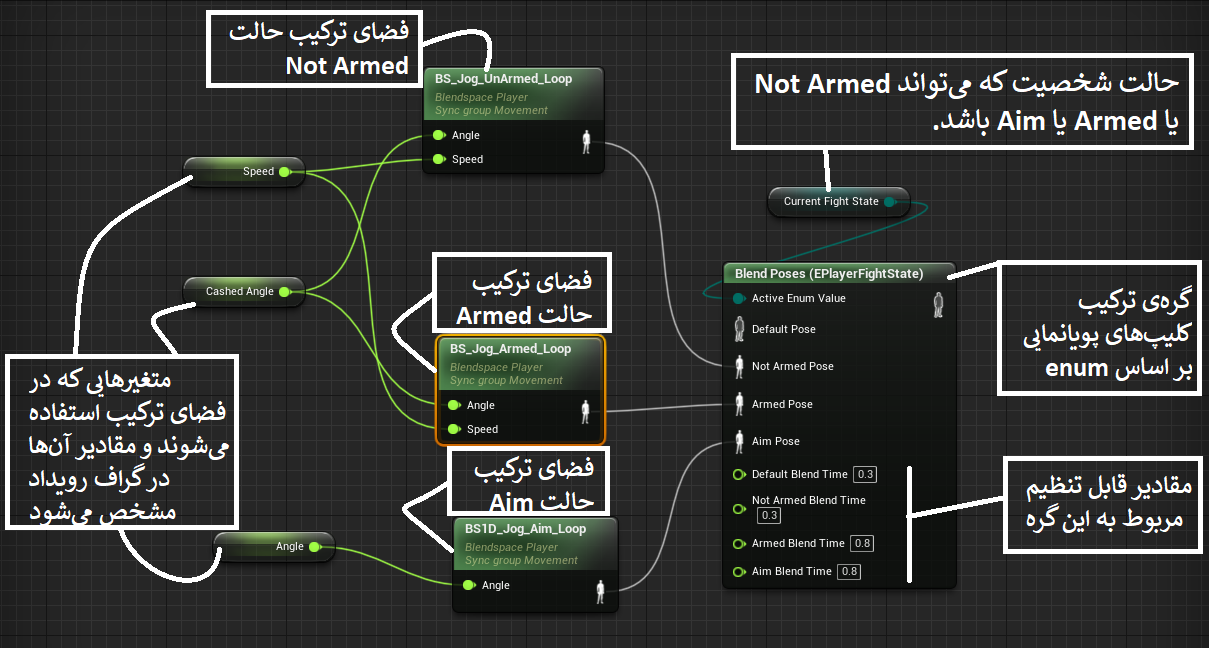
\includegraphics[width=\textwidth,height=8cm,keepaspectratio]{Figures/Ch3/EnumBlendNode_WithArrow.png}}\hfill
	\caption{ مثال استفاده از گره‌ی ترکیب }
	\label{fig:EnumBlendNode_WithArrow}
\end{figure}

\subsection{ گره‌ی ترکیب لایه‌ای برای هر مفصل}

با استفاده از این گره‌ می‌توانیم کلیپ‌ پویانمایی را بر روی 
مفاصل محدودی از اسکلت اجرا کنیم.
به عنوان مثال فرض کنید یک کلیپ پویانمایی مربوط به مشت زدن و کلیپ 
دیگری مربوط به حرکت شخصیت داریم. 
اگر بخواهیم از این دو کلیپ استفاده کنیم تا شخصیت در حال 
حرکت بتواند مشت هم بزند، می‌توان از این گره استفاده کرد.
با استفاده از این گره، می‌توان کلیپ مربوط به مشت زدن را تنها 
بر روی قسمت کمر به بالا‌‌‌ی شخصیت و کلیپ حرکت را بر 
روی کمر به پایین شخصیت اجرا کنیم.

\begin{figure}[ht]
	\centerline{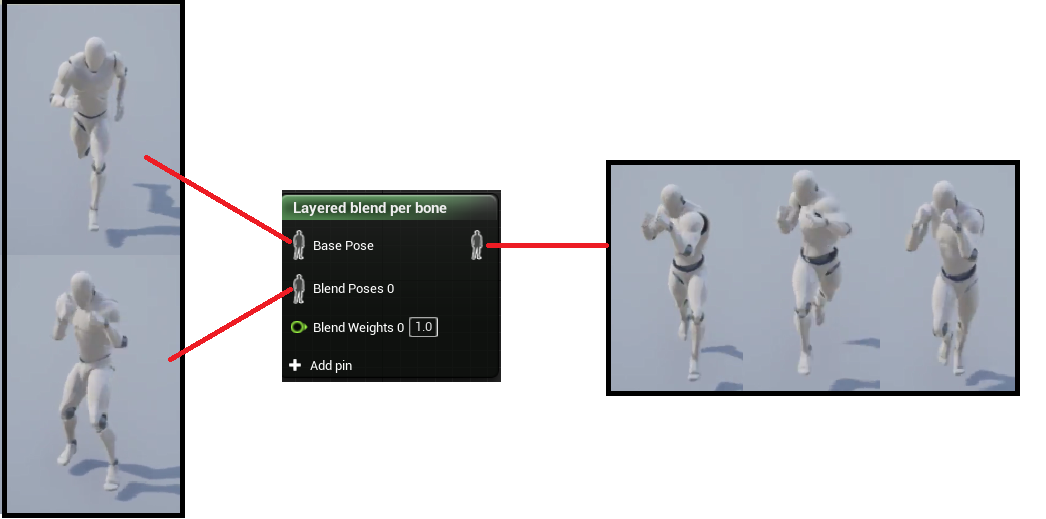
\includegraphics[width=\textwidth,height=8cm,keepaspectratio]{Figures/Ch3/LayeredBlendPerBone_WithArrow.png}}\hfill
	\caption{ اجرای کلیپ‌‌‌های پویانمایی بر روی مفاصل متفاوت }
	\label{fig:LayeredBlendPerBone_WithArrow}
\end{figure}

\cite{BlendNodeUnrealEngine}


\section{گره‌های کنترل اسکلت}

این گره‌ها امکان دستکاری مستقیم مفاصل موجود در اسکلت را فراهم می‌کنند.
مجموعه‌ی این گره‌ها شامل حل‌کننده‌های مختلف هستند که می‌توان به 
حل کننده‌ی 
\lr{IK}
به عنوان مثال اشاره کرد.
علاوه بر این بعضی از گره‌های مربوط به این قسمت، می‌توانند برای اعمال فیزیک بر روی 
مفاصل استفاده شوند.
\cite{SkeletalControlsUnrealEngine}

\section{گره‌های تبدیل فضا}

در موتور آنریل ژست‌ها می‌توانند در فضای محلی یا فضای مولفه قرار گیرند.
در فضای محلی مفاصل نسبت به والد خود قرار می‌گیرند، در صورتی که 
در فضای مولفه، مفاصل نسبت به مولفه‌ی مش اسکلتی 
\LTRfootnote{SkeletalMeshComponent}
قرار می‌گیرند.
اکثر گره‌ها با ژست‌ها در هنگامی که در فضای محلی قرار دارند، کار می‌کنند.
اما بعضی از گره‌های ترکیب و تمامی گره‌های کنترل اسکلت 
با ژست در فضای مولفه کار می‌کنند. بنابراین لازم از در مواقع لازم با استفاده از 
این گره، ژست اسکلت را از یک فضا به فضای دیگر منتقل کنیم.
\cite{ChangeSpaceUnrealEngine}

\begin{figure}[ht]
	\centerline{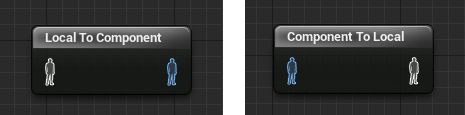
\includegraphics[width=\textwidth,height=8cm,keepaspectratio]{Figures/Ch3/ChnageSpaceNodes.png}}\hfill
	\caption{ گره‌های تبدیل حالت }
	\label{fig:ChnageSpaceNodes}
\end{figure}

\section{گره‌‌ی ماشین حالت}

ماشین‌های حالت، یک راه گرافیکی برای شکستن پویانمایی 
شخصیت‌ها به یک سری حالت را ارائه می‌دهند.
در آنریل می‌توان ماشین‌های حالت پیچیده و تو در تو بر اساس نیاز کاربران به وجود آورد.


\begin{figure}[ht]
	\centerline{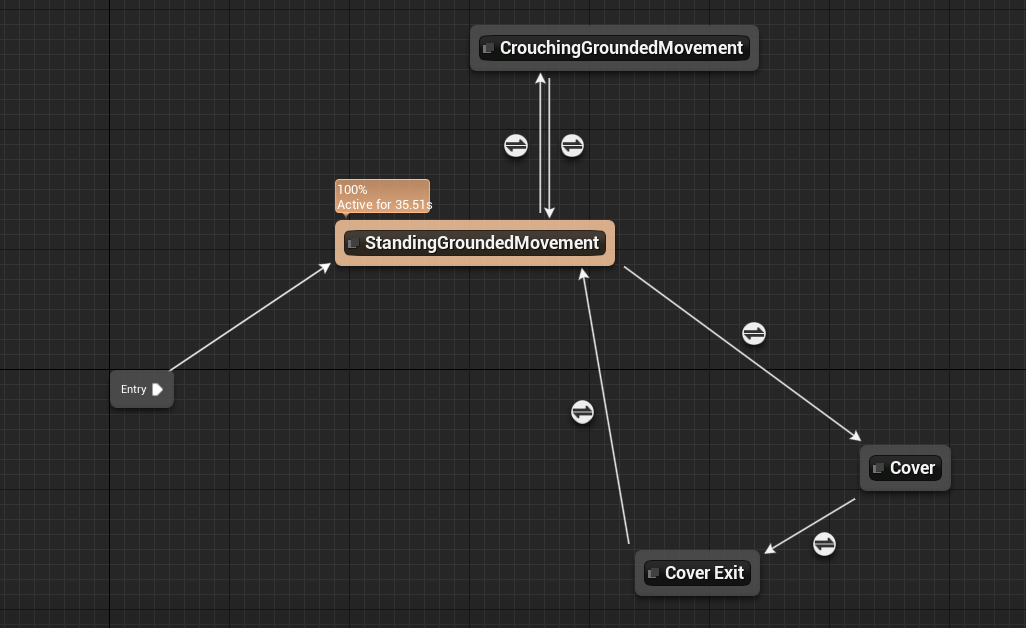
\includegraphics[width=\textwidth,height=8cm,keepaspectratio]{Figures/Ch3/AnimationStateMachine1.png}}\hfill
	\caption{ ماشین حالت برای حرکت شخصیت }
	\label{fig:AnimationStateMachine1}
\end{figure}

\begin{figure}[ht]
	\centerline{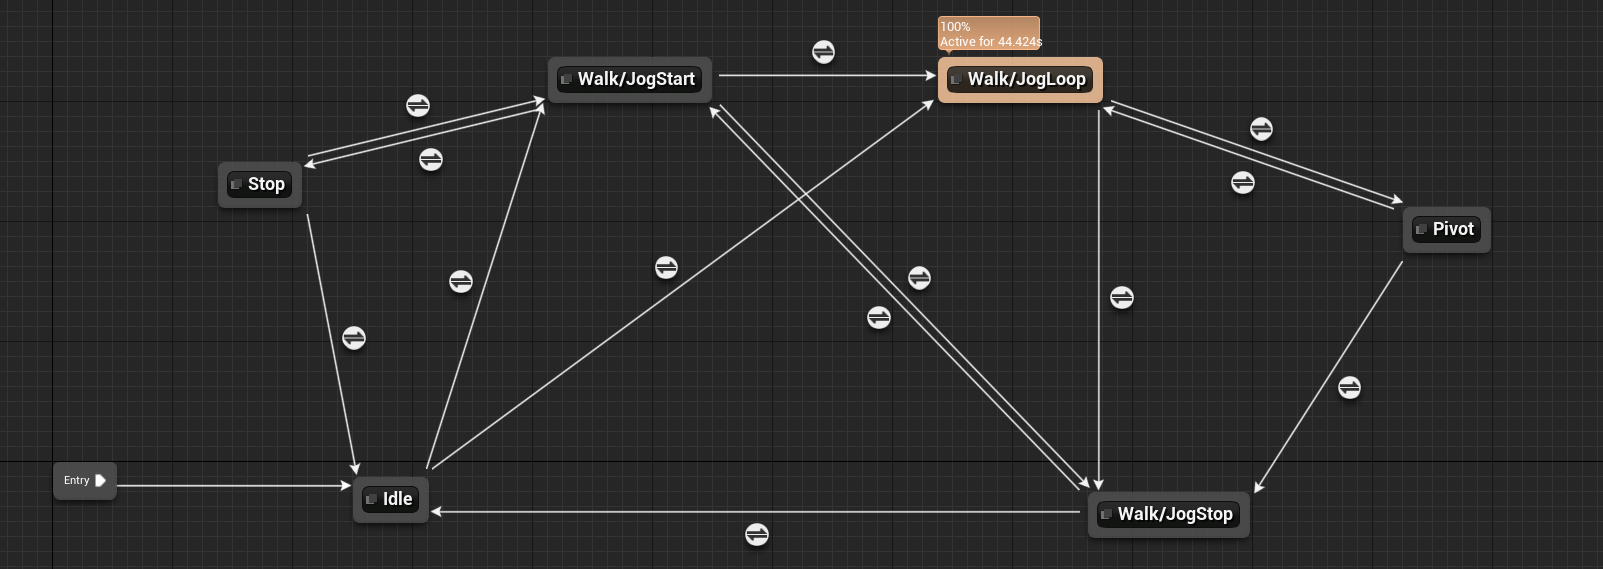
\includegraphics[width=\textwidth,height=8cm,keepaspectratio]{Figures/Ch3/AnimationStateMachine3.png}}\hfill
	\caption{ شخصیت ماشین حالت برای حرکت شخصیت در هنگام روی زمین قرار گرفتن  }
	\label{fig:AnimationStateMachine3}
\end{figure}

\section{نتیجه‌گیری}

در این فصل نگاهی بر موتور بازی‌سازی آنریل با تاکید بر گراف پویانمایی انداختیم.
همچنین توضیحات کاملی، درباره‌ی ویژگی‌هایی که گراف پویانمایی در اختیار کاربران می‌گذارد، آورده شد.
بنابراین آشنایی کافی با ابزار‌هایی که یک سیستم پویانمایی در اختیار کاربران می‌گذارد و 
اینکه این ابزارها در چه مواردی استفاده می‌شوند، پیدا کردیم.
حال برای درک بیشتر آنچه در داخل این سیسیتم‌ها اتفاق می‌افتد، به پیاده‌سازی یک سیستم پویانمایی از پایه می‌پردازیم.



